\chapter{Direct Memory Access}

The DMA engine can either write a specific byte to RAM or copy a set of bytes from one location in RAM to another. The DMA engine can also treat memory as being arranged either linearly (that is, as a certain number of consecutive locations) or as a rectangle (the data is a rectangular area of an image).

\section*{Linear Data}
Linear data (or ``1D'', if you prefer) is just a single block of sequential memory locations. When filling or copying data linearly, you need a destination address (and a source address if copying), and a count of bytes to copy. That is really all there is to it.

\section*{Rectangular Data}
Rectangular data (or ``2D'') is a bit more complicated and is meant to be working with image data. With a bitmap, the pixel bytes are arranged in memory left to right and top to bottom. If the image starts at address $a$ and is $w$ pixels wide, then the pixel at $(x, y)$ can be found at location $a + y \times w + x$. Rectangular fills and copies are meant to work on data that is arranged in this fashion. In this case, you can use DMA to fill or copy a rectangular area within that image. As with linear fills and copies, you will need a destination address (and source address if doing a copy), but instead of a count of bytes you need the width and height of the rectangular areas affected. But you need one other thing, too. You need to tell the DMA the geometry of the over-all image... you need to tell it the width of the image containing the rectangular areas. This is called the ``stride'' and effectively tells the DMA how many pixels to skip between lines when it finishes one line of the rectangle before getting to the next line.

\begin{table}[ht]
    \begin{center}
        \begin{tabular}{|c|c|c|c|c|c|c|c|c|c|} \hline
            Address & R/W & 7 & 6 & 5 & 4 & 3 & 2 & 1 & 0 \\\hline\hline
            \verb+0xDF00+ & R/W & START & \multicolumn{3}{|c|}{---} & INT\_EN & FILL & 2D & ENABLE \\ \hline
            \verb+0xDF01+ & W & FD7 & FD6 & FD5 & FD4 & FD3 & FD2 & FD1 & FD0 \\ \hline
            \verb+0xDF01+ & R & BUSY & \multicolumn{7}{|c|}{---}  \\ \hline\hline

            \verb+0xDF04+ & R/W & SA7 & SA6 & SA5 & SA4 & SA3 & SA2 & SA1 & SA0 \\ \hline
            \verb+0xDF05+ & R/W & SA15 & SA14 & SA13 & SA12 & SA11 & SA10 & SA9 & SA8 \\ \hline
            \verb+0xDF06+ & R/W & \multicolumn{5}{|c|}{---} & SA18 & SA17 & SA16 \\ \hline\hline

            \verb+0xDF08+ & R/W & DA7 & DA6 & DA5 & DA4 & DA3 & DA2 & DA1 & DA0 \\ \hline
            \verb+0xDF09+ & R/W & DA15 & DA14 & DA13 & DA12 & DA11 & DA10 & DA9 & DA8 \\ \hline
            \verb+0xDF0A+ & R/W & \multicolumn{5}{|c|}{---} & DA18 & DA17 & DA16 \\ \hline
        \end{tabular}
    \end{center}
    \caption{DMA Registers (Part 1)}
    \label{tab:dma_reg}
\end{table}

\begin{table}[ht]
    \begin{center}
        \begin{tabular}{|c|c|c|c|c|c|c|c|c|c|} \hline
            Address & R/W & 7 & 6 & 5 & 4 & 3 & 2 & 1 & 0 \\\hline\hline
            \verb+0xDF0C+ & R/W & CNT7 & CNT6 & CNT5 & CNT4 & CNT3 & CNT2 & CNT1 & CNT0 \\ \hline
            \verb+0xDF0D+ & R/W & CNT15 & CNT14 & CNT13 & CNT12 & CNT11 & CNT10 & CNT9 & CNT8 \\ \hline
            \verb+0xDF0E+ & R/W & \multicolumn{5}{|c|}{---} & CNT18 & CNT17 & CNT16 \\ \hline\hline

            \verb+0xDF0C+ & R/W & W7 & W6 & W5 & W4 & W3 & W2 & W1 & W0 \\ \hline
            \verb+0xDF0D+ & R/W & W15 & W14 & W13 & W12 & W11 & W10 & W9 & W8 \\ \hline
            \verb+0xDF0E+ & R/W & H7 & H6 & H5 & H4 & H3 & H2 & H1 & H0 \\ \hline
            \verb+0xDF0F+ & R/W & H15 & H14 & H13 & H12 & H11 & H10 & H9 & H8 \\ \hline\hline

            \verb+0xDF10+ & R/W & SS7 & SS6 & SS5 & SS4 & SS3 & SS2 & SS1 & SS0 \\ \hline
            \verb+0xDF11+ & R/W & SS15 & SS14 & SS13 & SS12 & SS11 & SS10 & SS9 & SS8 \\ \hline

            \verb+0xDF12+ & R/W & SD7 & SD6 & SD5 & SD4 & SD3 & SD2 & SD1 & SD0 \\ \hline
            \verb+0xDF13+ & R/W & SD15 & SD14 & SD13 & SD12 & SD11 & SD10 & SD9 & SD8 \\ \hline
        \end{tabular}
    \end{center}
    \caption{DMA Registers (Part 2)}
    \label{tab:dma_reg_2}
\end{table}


\begin{description}
    \item[START] set to trigger the DMA

    \item[INT\_EN] enables triggering an interrupt when DMA is complete

    \item[FILL] when set, DMA will write a specific byte to memory. When clear, DMA will copy data from a source address to the destination address

    \item[2D] when set, DMA copies or fills a rectangular region of memory. When clear, DMA copies or fills a certain number of sequential bytes

    \item[ENABLE] set to enable DMA

    \item[FD] the byte to be written to memory when FILL is set

    \item[BUSY] status bit set when DMA is busy copying data

    \item[SA] the 19 bit source address (must be a location in the first 512KB of RAM). Only relevant when FILL is clear.

    \item[DA] the 19 bit destination address (must be a location in the first 512KB of RAM)

    \item[CNT] the number of bytes to copy (only available when 2D is clear)

    \item[W] the width of the rectangle of data to copy (only available when 2D is set)

    \item[H] the height of the rectangle of data to copy (only available when 2D is set)

    \item[SS] the width of the ``stride'' for the source bitmap (only available for 2D copy operations)

    \item[SD] the width of the ``stride'' for the destination bitmap (only available when 2D is set)
\end{description}

The term ``stride'' might be a little confusing. It is a concept only relevant for 2D DMA operations. For 2D operations, the DMA engine is always copying or filling a rectangular area of a given width and height. The width of the rectangle need not be the full size of the overall bitmap image. If a program performs a DMA operation on a $32 \times 32$ area of the screen, the DMA engine will need to skip many pixels on each affected line. Thus, the program needs to inform the DMA engine how many pixels wide the bitmap is. For example, if a program is filling $32 \times 32$ rectangle in a $320 \times 240$ bitmap, it needs to tell the DMA engine that the width of the bitmap is 320. This number is the ``stride'' for the operation. The DMA engine will operate on 32 pixels, then skip $320 - 32$ pixels to get to the next set of 32 pixels to copy or fill. Figure~\ref{fig:dma_2d} illustrates how the various addresses, sizes, and strides work in the case of a 2D copy operation.

For 2D fill operations, only the destination stride (SD) is needed. The destination stride specifies how wide the bitmap being altered is. For 2D copy operations, both the destination stride and the source stride (SS) are needed. The source stride specifies how wide the bitmap is that provides the source data. Why would you ever have a source and destination stride be different? As a simple example, let's say a program needs to copy graphical font data to a bitmap for the screen in $320 \times 240$ mode. The characters are in cells that are 8 pixels wide by 16 pixels deep, and that the characters are arranged vertically. So the over all image for the characters is 8 pixels wide by 4,096 pixels high. In that case, the source stride is 8, but the destination stride is 320 (since it is the bitmap for the full screen).

\begin{figure}[ht]
    \begin{center}
        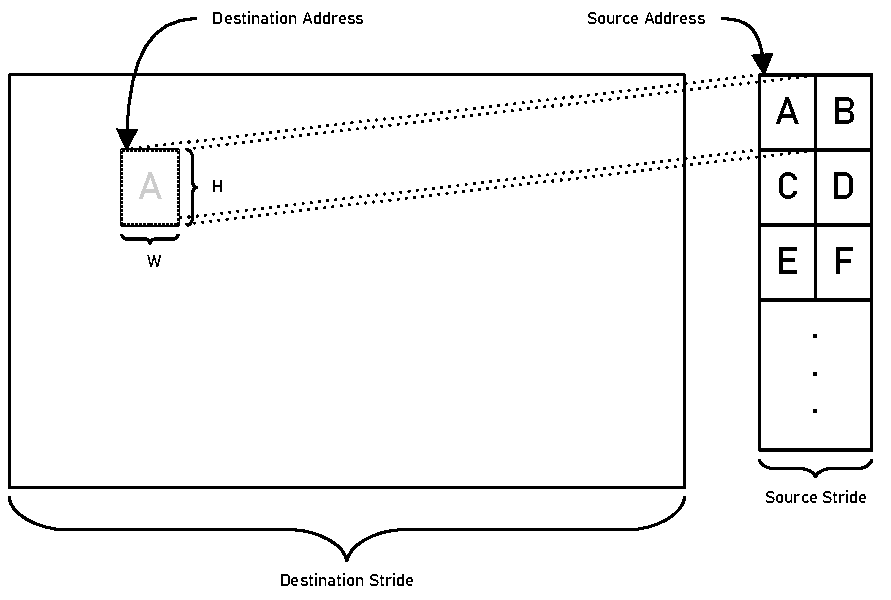
\includegraphics[scale=0.75]{images/f256_dma_2d.pdf}
    \end{center}
    \caption{A 2D Copy DMA Operation}
    \label{fig:dma_2d}
\end{figure}


\example{Using DMA to Fill a Bitmap}
\label{ex:dma}

In this example, we will use the 1D fill operation to set the bitmap shown on the screen to a set color. Note that the full example code includes the various setup operations for the bitmap mode and the graphics CLUTs, which are exactly the same as were used in the bitmap example (see page~\ref{ex:bitmap}).

\begin{verbatim}
DMA_CTRL = $DF00                ; DMA Control Register
DMA_CTRL_START = $80            ; Start the DMA operation
DMA_CTRL_FILL = $04             ; DMA is a fill operation
DMA_CTRL_ENABLE = $01           ; DMA engine is enabled

DMA_STATUS = $DF01              ; DMA status register (Read Only)
DMA_STAT_BUSY = $80             ; DMA engine is busy with an operation

DMA_FILL_VAL = $DF01            ; Byte value to use for fill operations

DMA_DST_ADDR = $DF08            ; Destination address (system bus)
DMA_COUNT = $DF0C               ; Number of bytes to fill or copy

bitmap_base = $10000            ; The base address of our bitmap

bitmap_width = 320              ; The size of our bitmap
bitmap_height = 240
bitmap_size = bitmap_width*bitmap_height
\end{verbatim}

First, we need to enable the DMA engine and set it up for a fill operation:

\begin{verbatim}
            lda #DMA_CTRL_FILL | DMA_CTRL_ENABLE
            sta DMA_CTRL
\end{verbatim}

Next, we provide the value to fill:

\begin{verbatim}
            lda #$ff
            sta DMA_FILL_VAL    ; We will fill the screen with $FF
\end{verbatim}

Then we need to provide the destination address:

\begin{verbatim}
            lda #<bitmap_base   ; Our bitmap will be the destination
            sta DMA_DST_ADDR
            lda #>bitmap_base
            sta DMA_DST_ADDR+1
            lda #`bitmap_base
            and #$03
            sta DMA_DST_ADDR+2
\end{verbatim}

Next, we provide the number of bytes to write:

\begin{verbatim}
            lda #<bitmap_size   ; We will write 320*240 bytes
            sta DMA_COUNT
            lda #>bitmap_size
            sta DMA_COUNT+1
            lda #`bitmap_size
            sta DMA_COUNT+2
\end{verbatim}

Finally, we flip the START flag to trigger the DMA operation and wait for it to complete:

\begin{verbatim}
            lda DMA_CTRL
            ora #DMA_CTRL_START
            sta DMA_CTRL

wait_dma:   lda DMA_STATUS      ; Wait until DMA is not busy
            and #DMA_STAT_BUSY
            cmp #DMA_STAT_BUSY
            beq wait_dma

            stz DMA_CTRL        ; Turn off the DMA engine
\end{verbatim}

\example{Using DMA to Fill a Rectangle}
\label{ex:dma_2d}

We can extend our 1D DMA example to draw a 2D rectangle at a given coordinate on the screen. In this example, we will calculate the starting address based on coordinates using the assembler's built-in math functions for constants. In general, a program will need to calculate these values at runtime and could use the built-in integer math coprocessor.

We will need to use some different registers to specify the size and layout of the rectangular area. These registers overlap the registers used in the 1D case. The first two replace the \verb+DMA_COUNT+ register to give the width and height of the rectangle. The second specifies the stride for the destination bitmap (for copying, there is a source stride as well that can be different from the destination stride):

\begin{verbatim}
            DMA_WIDTH = $DF0C               ; Width of rectangle (16-bit)
            DMA_HEIGHT = $DF0E              ; Height of rectangle (16-bit)
            DMA_STRIDE_DST = $DF12          ; Stride of the destination (16-bit)
\end{verbatim}

We start off very similar to the 1D fill and just turn on the flag for 2D DMA:

\begin{verbatim}
            lda #DMA_CTRL_FILL | DMA_CTRL_2D | DMA_CTRL_ENABLE
            sta DMA_CTRL
\end{verbatim}

We can then calculate the starting address, using the base address of the bitmap and a starting coordinate of $(100, 40)$:

\begin{verbatim}
            lda #<(bitmap_base + 320 * 40 + 100)
            sta DMA_DST_ADDR
            lda #>(bitmap_base + 320 * 40 + 100)
            sta DMA_DST_ADDR+1
            lda #`(bitmap_base + 320 * 40 + 100)
            sta DMA_DST_ADDR+2
\end{verbatim}

Next, we set the value to write into the bitmap fill area:

\begin{verbatim}
            lda #$30
            sta DMA_FILL_VAL    ; We will fill the screen with $30     
\end{verbatim}

A difference from 1D is that the size of the fill is a width and a height, so we provide the width and height of the rectangle we want to draw. In this case, we are setting it to $(100, 30)$:

\begin{verbatim}
            lda #100            ; Size of rectangle is (100,30)
            sta DMA_WIDTH
            stz DMA_WIDTH+1
            lda #30
            sta DMA_HEIGHT
            stz DMA_HEIGHT+1
\end{verbatim}

For 2D DMA operations, we need to provide the ``stride''. This is the width of the overall bitmap into which the DMA operation is writing. In this case, we are updating a bitmap that is the full screen, so we set the destination stride to 320:

\begin{verbatim}
            lda #<bitmap_width  ; Set the width of the destination bitmap for 2D DMA
            sta DMA_STRIDE_DST
            lda #>bitmap_width
            sta DMA_STRIDE_DST+1
\end{verbatim}

And then we can start the DMA operation and wait for it to complete:

\begin{verbatim}
            lda DMA_CTRL
            ora #DMA_CTRL_START
            sta DMA_CTRL

wait_dma2d: lda DMA_STATUS      ; Wait until DMA is not busy
            and #DMA_STAT_BUSY
            cmp #DMA_STAT_BUSY
            beq wait_dma2d
\end{verbatim}
